\documentclass[a4paper]{article}
\usepackage[spanish]{babel}
\usepackage[letterpaper,top=2cm,bottom=2cm,left=3cm,right=3cm,marginparwidth=1.75cm]{geometry}
\usepackage{amsmath}
\usepackage{graphicx}
\usepackage{authblk}
\usepackage{url}


\title{Apphelion, una aplicación para simular la trayectoria solar y la incidencia lumínica sobre viviendas}

\date{}
\author{Dr. Matías Micheletto}
\affil{Sendevo Software, Bahía Blanca (8000), Buenos Aires, Argentina.}
\affil{\texttt{holasendevo@gmail.com}}


\begin{document}
\maketitle 

\begin{abstract} 
\noindent En términos de arquitectura, la orientación de viviendas y edificaciones es fundamental para mejorar aspectos relacionados con la eficiencia energética, la comodidad habitacional y el aprovechamiento de la luz natural. Otros factores de diseño que pueden influir en estos aspectos pueden ser la ubicación de plantaciones o la extensión de techos y tejados mediante aleros, también denominados tejaroces o socarrenes. Para comprender la trayectoria solar y la incidencia de la misma sobre, no sólo las construcciones sino también paneles solares, en particular en latitudes alejadas del ecuador terrestre y durante las distintas épocas del año, el cambio del ángulo de incidencia del sol puede variar de manera considerable. En este artículo se detallan las fórmulas empleadas en cartas solares para calcular determinísticamente la posición del sol en el cielo en función de la ubicación geográfica y la fecha y hora. Se presenta la implementación de un software que permite simular la trayectoria solar y visualizar su efecto sobre modelos tridimencionales.
\end{abstract}

%\keywords{aplicaciones móviles; arquitectura; carta solar; vivienda; ingeniería civil}\\

\section{Introducción}

La trayectoria solar se refiere al camino que sigue el sol a lo largo del día y a lo largo del año. Este recorrido varía según la ubicación geográfica y la estación del año. Comprender la trayectoria solar permite a los arquitectos y diseñadores optimizar la orientación de los edificios para maximizar el aprovechamiento de la luz natural y minimizar la dependencia de la iluminación artificial y los sistemas de climatización.

La correcta orientación de una construcción puede aumentar significativamente la eficiencia energética \cite{salazar2014, wang2023}, reduciendo los costos de calefacción, refrigeración e iluminación. Por ejemplo, orientar las ventanas principales hacia el sur en el hemisferio norte y hacia el norte en el hemisferio sur permite capturar la mayor cantidad de luz solar durante el invierno, mientras que al mismo tiempo se evita el sobrecalentamiento en verano, siempre y cuando se disponga de extensiones en el techo a modo de aleros, para crear sombra sobre estas aberturas.

En el caso de paneles solares ocurre algo similar. Para aprovechar al máximo la generación de energía eléctrica, los vectores normales de sus superficies de captación debe apuntar hacia la posición del sol \cite{zalamea2023}. También es posible emplear dispositivos de seguimiento solar, los cuales cuentan con sensores que detectan la posición del sol, para orientar los paneles automáticamente. En el caso de disponer los datos de trayectoria solar en función de la época del año, puede evitarse el empleo de sensores, incluso de sistemas automáticos, sino que se ajusta manualmente la inclinación del panel en función de la estación, el mes o incluso semana \cite{ou2014}.

En este artículo se resumen los cálculos que intervienen en la determinación de la posición del sol en función de la ubicación e instante del año en que se encuentra cierto observador y la implementación de estas ecuaciones en un software multiplataforma para simular la incidencia del sol sobre superficies de modelos tridimensionales.

\section{Carta solar}

La posición del sol en el cielo tal como la ve un observador en la tierra depende de varios factores como la ubicación geográfica, la fecha y la hora del día. La grilla terrestre, demarcada mediante trazados verticales y horizontales a lo largo del globo, permite referenciar ubicaciones en cualquier parte del planeta. La medida de los ángulos longitudinales respecto a la hora del día tiene que ver con ciertas convenciones que fueron definidas históricamente, por lo que para realizar los cálculos pertinentes es necesario incorporar una carta tabulada a modo contar con todos los datos.

En astronomía, el ángulo de declinación del sol es la distancia angular norte o sur del ecuador celeste. Una de las fórmulas utilizadas para calcular la declinación del sol está dada por

\begin{equation}\label{eq:declinacion}
    \delta = 23.45 \cdot \sin \left(\frac{360}{365.25}\cdot \left(N+10\right)  \right)\text{,}
\end{equation}

donde 
\begin{itemize}
    \item $\delta$ es el valor de declinación en grados.
    \item N es el número de días desde el comienzo del año.
\end{itemize}

Por otro lado, el acimut del sol es la distancia angular a lo largo del horizonte medido en sentido horario desde el norte. Este ángulo va cambiando a lo largo del día a medida que el sol cruza el cielo. El acimut se puede calcular, para el caso del sol, a partir de la siguiente fórmula,

\begin{equation}\label{eq:acimut}
    \cos\left(\theta\right) = \frac{\sin\left(\delta\right)\cdot \cos\left(\phi\right) - \cos\left(H\right)\cdot\cos\left(\delta\right)\cdot\sin\left(\phi\right)}{\sin\left(\theta_s\right)}\text{,}
\end{equation}

donde
\begin{itemize}
    \item $\theta$ es el ángulo cenital solar $\left(90^o - \text{ángulo de elevación solar} \right)$.
    \item $\delta$ el la declinación del sol.
    \item $\phi$ es la latitud del observador.
    \item $H$ es el ángulo horario del sol que se calcula como la diferencia de tiempo por $15^o$ $\left( \Delta T \cdot 15^o \right)$.
    \item $\theta_s$ es el coseno del ángulo cenital solar.
\end{itemize}

Existen modelos más complejos que incluyen otros factores para incorporar correcciones de manera de obtener estimaciones más exactas. A los efectos de la funcionalidad que se pretende cubrir con la aplicación en cuestión, las aproximaciones presentadas aquí son suficientes.

\section{Materiales y métodos}

Pensando el lograr compatibilidad multiplataforma, la aplicación se construye íntegramente mediante lenguaje de programación web. Por lo que la elección de la tecnología se basa no sólo en la portabilidad sino en que permite incorporar tanto la implementación de la simulación como la capa de visualización de datos en una misma base de código.

El proyecto se organiza en distintas etapas. Se parte de un núcleo para contener el modelo de negocio, el cual incluye la implementación de los algoritmos de simulación. En un esquema de \textit{Clean Architecture} \cite{cleanarch}, este esquema se incluye en la capa central, donde son definidas las entidades del modelo.

A continuación se define una capa para el diseño de la interfaz gráfica, donde se separa la visualización de la información en tres secciones, una para la selección de la ubicación, otra para visualizar la carta solar y una tercera para simular la iluminación solar sobre un modelo 3D. En la parte superior se cuenta con un menú compuesto por todos los controles necesarios para la simulación, así como los desplegables para establecer ciertos parámetros relacionados con la configuración de la visualización o la selección de la fecha y hora.

Finalmente se programó un módulo para la importación de un modelo 3D y la renderización del mismo en la escena de simulación. En las siguientes subsecciones se detallan las principales consideraciones al momento de realizar la implementación de este software.

\subsection{Algoritmos}

El código de implementación de los algoritmos de cálculo se dividen en distintas secciones dependiendo de la funcionalidad. El dato de entrada que requiere el algoritmo de cálculo incluye principalmente la ubicación geográfica. A partir de esta información se calcula la trayectoria solar a lo largo de todo el año mediante las ecuaciones \ref{eq:declinacion} y \ref{eq:acimut}, haciendo un barrido de muestreo por las distintas fechas y horarios. Esto permite generar la tabla solar anual y la tabla solar diaria, cuyos datos son empleados para generar los gráficos de horas de luz, las trayectorias y el cálculo de proyecciones de sombras, entre otros.

Realizar el procesamiento de la lista de datos es computacionalmente intensivo y al ejecutar esta rutina como proceso de la misma aplicación, provoca demora y bloqueo de la aplicación. Una manera de evitar eso es usar \textit{service workers}, los cuales son procesos que se ejecutan en segundo plano. Una manera de acelerar la ejecución de los procesos en paralelo, es empleando rutinas de \textit{WebAssembly} (\textit{WASM}, por sus siglas en inglés), el cual es un lenguaje de bajo nivel que el navegador puede ejecutar a mayor velocidad que con \textit{JavaScript}.

Si bien se puede generar código \textit{WASM} a partir de la compilación de varios lenguaje de programación como \textit{Rust}, \textit{C/C++} o \textit{AssemblyScript}, por una cuestión de familiaridad con el entorno, se eligió \textit{C/C++} y \textit{Emscripten}\footnote{https://emscripten.org/} como compilador.

Los módulos compilados se pueden importar directamente desde el código web para intercambiar información en varios formatos, lo que permite enviar los datos de ubicación geográfica y recibir los arreglos con datos de la trayectoria solar. Este esquema acelera el procesamiento y mejora la experiencia del usuario, al calcular la carta solar a medida que se desplaza la ubicación sobre el mapa.

\subsection{Visualización}

La interfaz gráfica se implementó con distintas librerías. Con \textit{jQuery} \footnote{https://jquery.com/} se realiza el intercambio de variables ente los métodos de procesamiento y los elementos del documento, como los controles y formularios. Para la definición de estilos se utilizó \textit{Bootstrap} \footnote{https://getbootstrap.com/}, que provee un esquema completo para estilizar y alinear componentes de la ventana, entre otras funciones.

El mapa que muestra la ubicación sobre la que se calcula la carta solar se realizó con \textit{Leaflet} \footnote{https://leafletjs.com/}, que provee un marco para mostrar información geográfica extraida de \textit{OpenStreetMap}\footnote{https://www.openstreetmap.org/}.

\begin{figure}[ht]
    \centering
    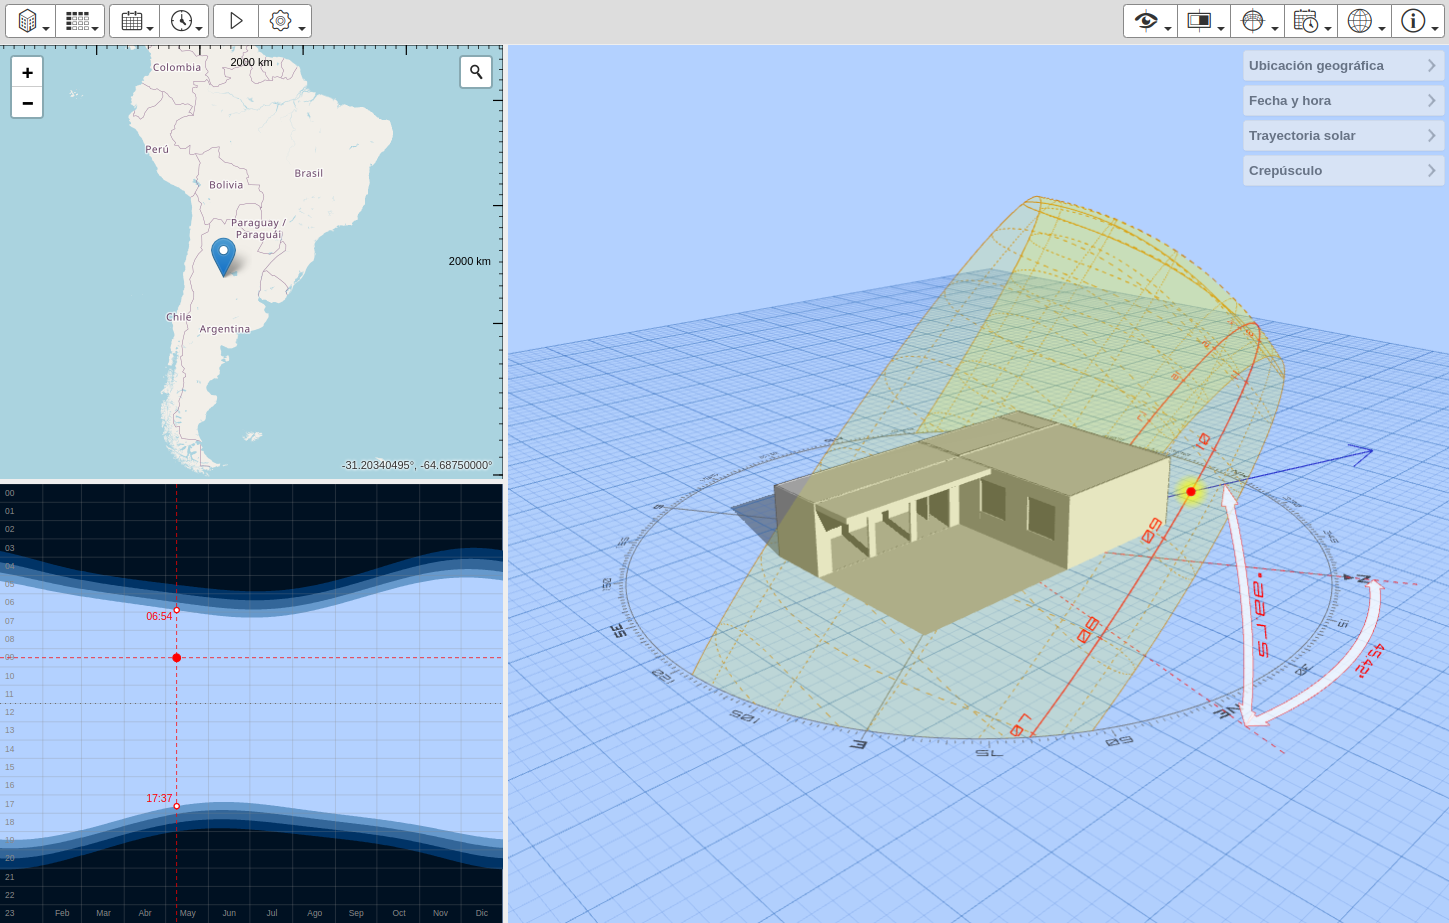
\includegraphics[width=\textwidth]{images/screenshot.png}
    \caption{Captura de pantalla.}
    \label{fig:screenshot}
\end{figure}

Para ilustrar el modelo 3D de construcciones como casas u otras edificaciones, se valió de la librería \textit{Three.js} \footnote{https://threejs.org/} y finalmente, para la presentación de la gráfica que muestra la duración del día se utilizó \textit{D3} \footnote{https://d3js.org/}.

\subsection{Importación de modelos 3D}
Una función relevante de la aplicación es la posibilidad de importar modelos 3D de construcciones. Los formatos aceptados son OBJ, PLY o STL, de los cuales, los primeros dos son preferibles al contar con información de texturas y colores. Los archivos importados son procesados para ser convertidos al formato \textit{JSON} que utiliza la librería \textit{Three.js}.

\subsection{Distribución}
La distribución del software se refiere a los medios por los cuales el mismo puede ser accedido por los distintos usuarios. Por cuestiones de seguridad, siempre se utilizan sitios de descarga seguros, los cuales implican direcciones de \textit{URL} de reputación comprobada, como tiendas de aplicaciones oficiales o sitios web con certificado \textit{SSL}. 

\begin{figure}[ht]
    \centering
    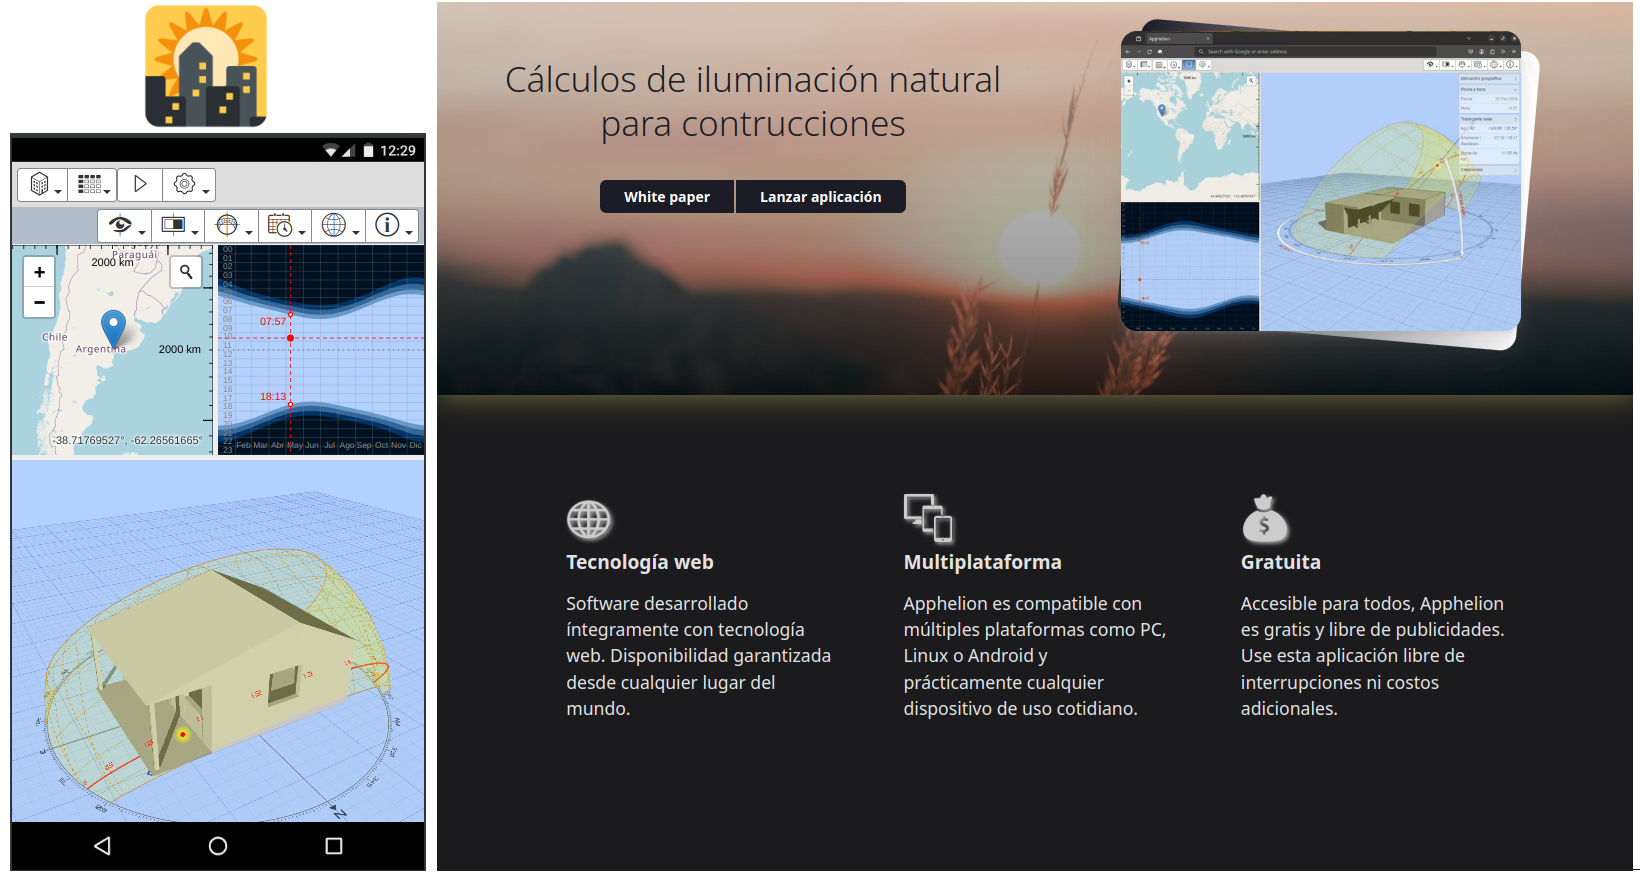
\includegraphics[width=\textwidth]{images/landing.png}
    \caption{Logotipo (Arriba a la izquierda), app móvil (abajo a la izquerda) y \textit{landing page} (derecha).}
    \label{fig:landing}
\end{figure}

El acceso al software \textit{Apphelion} se puede realizar a través de tres medios disponibles: el sitio web de la aplicación con posibilidad de instalación como \textit{PWA}, la tienda de aplicaciones de \textit{Android}\textregistered y por medio de archivos ejecutables tanto para \textit{Windows}\textregistered como para \textit{Linux} accesible a través de la página oficial del desarrollador. Para el caso de la compilación de la aplicación al formato ejecutable de \textit{Android}\textregistered (\textit{.apk}), se utiliza un esquema híbrido, el cual puede ser llevado a cabo con el \textit{framework} \textit{Capacitor.js} \footnote{https://capacitorjs.com/}. Para el caso de aplicaciones simples, este es un esquema que ha resultado práctico en anteriores desarrollos \cite{ref_criollo, ref_campero, ref_agrario}. La aplicación puede ser luego distribuida en la tienda de aplicaciones \textit{Google Play}\textregistered. De manera similar, se emplea \textit{Electron.js} \footnote{https://www.electronjs.org/es/} para la compilación del software para PC.

\subsection{Branding}
La etimología del producto se basa en la combinación de las palabras ``App'' que es la abreviatura de aplicación y ``Helion'', que es una variación de ``Helios'', quien fuera un personaje de la mitología griega que simboliza el sol. En otros casos como en el contexto de la astronomía, la palabra ``Helion'' hace referencia al cuerpo celeste alrededor del cual orbita la Tierra. Respecto del diseño de logo e identidad del software Apphelion, se emplea, a modo e ícono, una imagen simplificada del sol en un amanecer entre edificios de ciudad. A la fecha de redacción de este trabajo, la interfaz gráfica presenta un estilo de tema claro, sin la opción de alternar a un tema oscuro.

En la figura \ref{fig:landing} se muestra el logotipo diseñado para la aplicación, que se encuentra presente como icono de página (favicono) de la versión web, una captura de pantalla de la versión móvil y una captura de pantalla del encabezado de la página de aterrizaje o \textit{landing page}, la cual ilustra las principales características de la aplicación y el flujo de trabajo.

\section{Conclusión}
La implementación de los cálculos de trayectoria solar en un software como el planteado en este artículo y sumado a la posibilidad de renderizar un modelo 3D para visualizar la iluminación natural sobre el mismo, hacen de esta herramienta un sistema sustancialmente útil durante el diseño de una vivienda, como su orientación, la dirección y dimensión de aberturas, las estructuras de sombra como aleros, cobertizos y árboles, entre muchas otras.

La elección de la tecnología web como base para el proyecto Apphelion se basa en que ofrece una serie de beneficios significativos para la implementación de software. Desde sus inicios, se enfoca en la accesibilidad y compatibilidad, permitiendo a los usuarios acceder al software desde cualquier dispositivo con conexión a Internet. Esto fomenta la colaboración y la flexibilidad en el trabajo. Además, la tecnología web simplifica el proceso de actualización y mantenimiento, ya que los cambios pueden implementarse de forma centralizada y sin necesidad de descargar actualizaciones manualmente. Asimismo, reduce los costos de infraestructura, ya que no se requieren instalaciones complejas en los dispositivos de los usuarios.

A modo de trabajo futuro resta implementar los cálculos de radiación para determinar la cantidad de energía solar disponible sobre cada una de las superficies del modelo 3D. Si bien es un factor que depende en buena medida de los materiales de dichas superficies, es una herramienta más que aporta certezas respecto de qué inclinación y orientación deben tener objetos como techos, paredes, paneles solares y demás. Si bien este desarrollo representa un producto lucrativo, a la fecha de redacción de este artículo, el software Apphelion está disponible de forma libre y gratuita, sin publicidades ni requisitos de suscripción, entre otras limitaciones.

\bibliographystyle{acm}
\bibliography{bib}

\end{document}